\section{The Arrival Problem}
The arrival problem, first described in \citep{arrivalBasic} is fundamentally
a reachability problem. The idea is, given a directed graph with
a particular structure and designated source and target vertex,
decide whether or not a particular walk starting at the source
ever reaches the target. A diagram of an example arrival graph is shown
in $\cref{arrivalDiagram}$.
\begin{definition}[Arrival Graph]
  An \emph{arrival graph} is a set of vertices $V$, a pair of
  vertices $s, t \in V$, and a pair of maps 
  $s_0, s_1 : V \to V$. 
\end{definition}
\begin{definition}[Arrival Walk]
  Let $(V, s, t, s_0, s_1)$ be an arrival graph. The \emph{arrival walk}
  on this graph is a sequence of vertices $(v_i)_{i \in \znn} \in V$
  such that $v_0 = s$, and $v_{i+1} = 
  \begin{cases} 
    s_0(v_i), & \text{$n_i$ even}\\  
    s_1(v_i), & \text{$n_i$ odd},
  \end{cases}$
  where $n_i$ is the number of times $v_i$ has appeared previously in
  the sequence.
\end{definition}
It is clear that the arrival walk for a particular arrival graph
is entirely defined by the structure of the graph, which is what
lead it to be called a zero player graph game in \citep{arrivalBasic}.
\begin{definition}[$\textsc{Arrival}$]
  The $\textsc{Arrival}$ problem is, given an arrival graph $(V, s, t, s_0, s_1)$,
  decide whether or not the arrival walk ever reaches $t$.
\end{definition}
\begin{figure}[h]
  \tikzset{every picture/.style={line width=0.75pt}} %set default line width to 0.75pt        

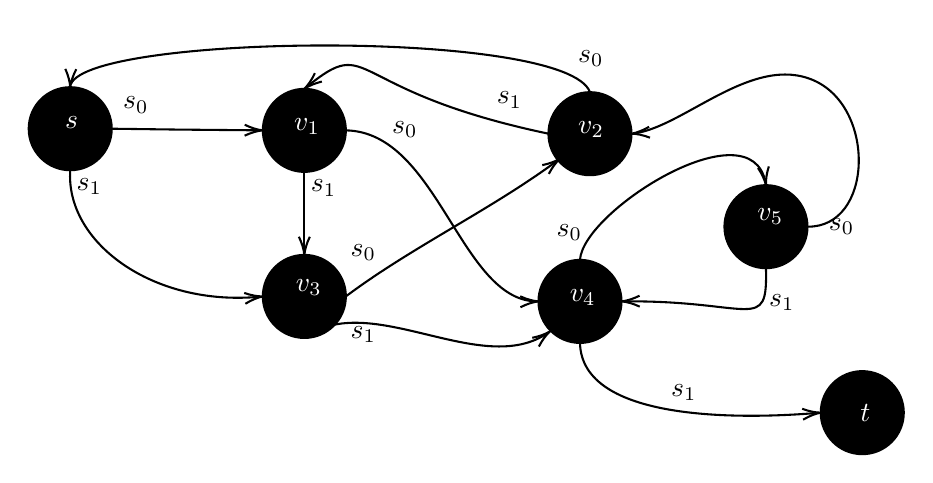
\begin{tikzpicture}[x=0.6pt,y=0.6pt,yscale=-1,xscale=1]
%uncomment if require: \path (0,300); %set diagram left start at 0, and has height of 300

%Shape: Circle [id:dp5495329281078569] 
\draw  [fill={rgb, 255:red, 0; green, 0; blue, 0 }  ,fill opacity=1 ] (32,49) .. controls (32,35.19) and (43.19,24) .. (57,24) .. controls (70.81,24) and (82,35.19) .. (82,49) .. controls (82,62.81) and (70.81,74) .. (57,74) .. controls (43.19,74) and (32,62.81) .. (32,49) -- cycle ;
%Straight Lines [id:da33331850965746734] 
\draw    (82,49) -- (121.98,49.53) -- (171,49.98) ;
\draw [shift={(173,50)}, rotate = 180.52] [color={rgb, 255:red, 0; green, 0; blue, 0 }  ][line width=0.75]    (10.93,-3.29) .. controls (6.95,-1.4) and (3.31,-0.3) .. (0,0) .. controls (3.31,0.3) and (6.95,1.4) .. (10.93,3.29)   ;
%Shape: Circle [id:dp8549825383964691] 
\draw  [fill={rgb, 255:red, 0; green, 0; blue, 0 }  ,fill opacity=1 ] (173,50) .. controls (173,36.19) and (184.19,25) .. (198,25) .. controls (211.81,25) and (223,36.19) .. (223,50) .. controls (223,63.81) and (211.81,75) .. (198,75) .. controls (184.19,75) and (173,63.81) .. (173,50) -- cycle ;
%Straight Lines [id:da15070581279870932] 
\draw    (198,75) -- (198,123) ;
\draw [shift={(198,125)}, rotate = 270] [color={rgb, 255:red, 0; green, 0; blue, 0 }  ][line width=0.75]    (10.93,-3.29) .. controls (6.95,-1.4) and (3.31,-0.3) .. (0,0) .. controls (3.31,0.3) and (6.95,1.4) .. (10.93,3.29)   ;
%Shape: Circle [id:dp4390825091110777] 
\draw  [fill={rgb, 255:red, 0; green, 0; blue, 0 }  ,fill opacity=1 ] (345,52) .. controls (345,38.19) and (356.19,27) .. (370,27) .. controls (383.81,27) and (395,38.19) .. (395,52) .. controls (395,65.81) and (383.81,77) .. (370,77) .. controls (356.19,77) and (345,65.81) .. (345,52) -- cycle ;
%Shape: Circle [id:dp9757305512769809] 
\draw  [fill={rgb, 255:red, 0; green, 0; blue, 0 }  ,fill opacity=1 ] (173,150) .. controls (173,136.19) and (184.19,125) .. (198,125) .. controls (211.81,125) and (223,136.19) .. (223,150) .. controls (223,163.81) and (211.81,175) .. (198,175) .. controls (184.19,175) and (173,163.81) .. (173,150) -- cycle ;
%Shape: Circle [id:dp6476109813645592] 
\draw  [fill={rgb, 255:red, 0; green, 0; blue, 0 }  ,fill opacity=1 ] (339,153) .. controls (339,139.19) and (350.19,128) .. (364,128) .. controls (377.81,128) and (389,139.19) .. (389,153) .. controls (389,166.81) and (377.81,178) .. (364,178) .. controls (350.19,178) and (339,166.81) .. (339,153) -- cycle ;
%Shape: Circle [id:dp9387189635111892] 
\draw  [fill={rgb, 255:red, 0; green, 0; blue, 0 }  ,fill opacity=1 ] (451,108) .. controls (451,94.19) and (462.19,83) .. (476,83) .. controls (489.81,83) and (501,94.19) .. (501,108) .. controls (501,121.81) and (489.81,133) .. (476,133) .. controls (462.19,133) and (451,121.81) .. (451,108) -- cycle ;
%Shape: Circle [id:dp6728900489022538] 
\draw  [fill={rgb, 255:red, 0; green, 0; blue, 0 }  ,fill opacity=1 ] (509,220) .. controls (509,206.19) and (520.19,195) .. (534,195) .. controls (547.81,195) and (559,206.19) .. (559,220) .. controls (559,233.81) and (547.81,245) .. (534,245) .. controls (520.19,245) and (509,233.81) .. (509,220) -- cycle ;
%Curve Lines [id:da06839655673782064] 
\draw    (223,50) .. controls (278.44,50.99) and (291.74,151.95) .. (337.6,153) ;
\draw [shift={(339,153)}, rotate = 178.78] [color={rgb, 255:red, 0; green, 0; blue, 0 }  ][line width=0.75]    (10.93,-3.29) .. controls (6.95,-1.4) and (3.31,-0.3) .. (0,0) .. controls (3.31,0.3) and (6.95,1.4) .. (10.93,3.29)   ;
%Curve Lines [id:da30024168681774177] 
\draw    (364,178) .. controls (364.99,225.52) and (461.05,224.04) .. (507.6,220.12) ;
\draw [shift={(509,220)}, rotate = 175.03] [color={rgb, 255:red, 0; green, 0; blue, 0 }  ][line width=0.75]    (10.93,-3.29) .. controls (6.95,-1.4) and (3.31,-0.3) .. (0,0) .. controls (3.31,0.3) and (6.95,1.4) .. (10.93,3.29)   ;
%Curve Lines [id:da031177664907863667] 
\draw    (370,27) .. controls (356.28,-11.22) and (69.81,-8.14) .. (57.41,22.11) ;
\draw [shift={(57,24)}, rotate = 271.79] [color={rgb, 255:red, 0; green, 0; blue, 0 }  ][line width=0.75]    (10.93,-3.29) .. controls (6.95,-1.4) and (3.31,-0.3) .. (0,0) .. controls (3.31,0.3) and (6.95,1.4) .. (10.93,3.29)   ;
%Curve Lines [id:da19551484489395188] 
\draw    (364,128) .. controls (365.79,98.44) and (466.95,34.79) .. (475.76,81.55) ;
\draw [shift={(476,83)}, rotate = 261.95] [color={rgb, 255:red, 0; green, 0; blue, 0 }  ][line width=0.75]    (10.93,-3.29) .. controls (6.95,-1.4) and (3.31,-0.3) .. (0,0) .. controls (3.31,0.3) and (6.95,1.4) .. (10.93,3.29)   ;
%Curve Lines [id:da5453571551089418] 
\draw    (345,52) .. controls (220.26,25.76) and (239.59,-8.8) .. (199.24,23.99) ;
\draw [shift={(198,25)}, rotate = 320.6] [color={rgb, 255:red, 0; green, 0; blue, 0 }  ][line width=0.75]    (10.93,-3.29) .. controls (6.95,-1.4) and (3.31,-0.3) .. (0,0) .. controls (3.31,0.3) and (6.95,1.4) .. (10.93,3.29)   ;
%Curve Lines [id:da7736997926226343] 
\draw    (223,150) .. controls (262.6,120.3) and (311.02,97.46) .. (350.8,67.9) ;
\draw [shift={(352,67)}, rotate = 143.13] [color={rgb, 255:red, 0; green, 0; blue, 0 }  ][line width=0.75]    (10.93,-3.29) .. controls (6.95,-1.4) and (3.31,-0.3) .. (0,0) .. controls (3.31,0.3) and (6.95,1.4) .. (10.93,3.29)   ;
%Curve Lines [id:da35489757719958615] 
\draw    (57,74) .. controls (54.03,117.56) and (106.93,156.22) .. (171.05,150.2) ;
\draw [shift={(173,150)}, rotate = 173.85] [color={rgb, 255:red, 0; green, 0; blue, 0 }  ][line width=0.75]    (10.93,-3.29) .. controls (6.95,-1.4) and (3.31,-0.3) .. (0,0) .. controls (3.31,0.3) and (6.95,1.4) .. (10.93,3.29)   ;
%Curve Lines [id:da7424500525745132] 
\draw    (198,175) .. controls (237.6,145.3) and (304.64,199.89) .. (344.79,171.87) ;
\draw [shift={(346,171)}, rotate = 143.13] [color={rgb, 255:red, 0; green, 0; blue, 0 }  ][line width=0.75]    (10.93,-3.29) .. controls (6.95,-1.4) and (3.31,-0.3) .. (0,0) .. controls (3.31,0.3) and (6.95,1.4) .. (10.93,3.29)   ;
%Curve Lines [id:da3132040250840804] 
\draw    (501,108) .. controls (540.44,108.6) and (542.5,36.73) .. (505,20) .. controls (468.25,3.6) and (426.87,47.76) .. (396.83,51.8) ;
\draw [shift={(395,52)}, rotate = 355.43] [color={rgb, 255:red, 0; green, 0; blue, 0 }  ][line width=0.75]    (10.93,-3.29) .. controls (6.95,-1.4) and (3.31,-0.3) .. (0,0) .. controls (3.31,0.3) and (6.95,1.4) .. (10.93,3.29)   ;
%Curve Lines [id:da9721751571878057] 
\draw    (476,133) .. controls (477,172.8) and (468.09,152.21) .. (390.18,152.99) ;
\draw [shift={(389,153)}, rotate = 359.27] [color={rgb, 255:red, 0; green, 0; blue, 0 }  ][line width=0.75]    (10.93,-3.29) .. controls (6.95,-1.4) and (3.31,-0.3) .. (0,0) .. controls (3.31,0.3) and (6.95,1.4) .. (10.93,3.29)   ;

% Text Node
\draw (87,28) node [anchor=north west][inner sep=0.75pt]   [align=left] {$\displaystyle s_{0}$};
% Text Node
\draw (52,40) node [anchor=north west][inner sep=0.75pt]  [color={rgb, 255:red, 255; green, 255; blue, 255 }  ,opacity=1 ] [align=left] {$\displaystyle s$};
% Text Node
\draw (59,77) node [anchor=north west][inner sep=0.75pt]   [align=left] {$\displaystyle s_{1}$};
% Text Node
\draw (249,43) node [anchor=north west][inner sep=0.75pt]   [align=left] {$\displaystyle s_{0}$};
% Text Node
\draw (190,41) node [anchor=north west][inner sep=0.75pt]  [color={rgb, 255:red, 255; green, 255; blue, 255 }  ,opacity=1 ] [align=left] {$\displaystyle v_{1}$};
% Text Node
\draw (200,78) node [anchor=north west][inner sep=0.75pt]   [align=left] {$\displaystyle s_{1}$};
% Text Node
\draw (361,0) node [anchor=north west][inner sep=0.75pt]   [align=left] {$\displaystyle s_{0}$};
% Text Node
\draw (361,43) node [anchor=north west][inner sep=0.75pt]  [color={rgb, 255:red, 255; green, 255; blue, 255 }  ,opacity=1 ] [align=left] {$\displaystyle v_{2}$};
% Text Node
\draw (224,117) node [anchor=north west][inner sep=0.75pt]   [align=left] {$\displaystyle s_{0}$};
% Text Node
\draw (191,138) node [anchor=north west][inner sep=0.75pt]  [color={rgb, 255:red, 255; green, 255; blue, 255 }  ,opacity=1 ] [align=left] {$\displaystyle v_{3}$};
% Text Node
\draw (224,166) node [anchor=north west][inner sep=0.75pt]   [align=left] {$\displaystyle s_{1}$};
% Text Node
\draw (348,105) node [anchor=north west][inner sep=0.75pt]   [align=left] {$\displaystyle s_{0}$};
% Text Node
\draw (356,144) node [anchor=north west][inner sep=0.75pt]  [color={rgb, 255:red, 255; green, 255; blue, 255 }  ,opacity=1 ] [align=left] {$\displaystyle v_{4}$};
% Text Node
\draw (417,201) node [anchor=north west][inner sep=0.75pt]   [align=left] {$\displaystyle s_{1}$};
% Text Node
\draw (512,101) node [anchor=north west][inner sep=0.75pt]   [align=left] {$\displaystyle s_{0}$};
% Text Node
\draw (469,95) node [anchor=north west][inner sep=0.75pt]  [color={rgb, 255:red, 255; green, 255; blue, 255 }  ,opacity=1 ] [align=left] {$\displaystyle v_{5}$};
% Text Node
\draw (476,147) node [anchor=north west][inner sep=0.75pt]   [align=left] {$\displaystyle s_{1}$};
% Text Node
\draw (531,213) node [anchor=north west][inner sep=0.75pt]  [color={rgb, 255:red, 255; green, 255; blue, 255 }  ,opacity=1 ] [align=left] {$\displaystyle t$};
% Text Node
\draw (312,25) node [anchor=north west][inner sep=0.75pt]   [align=left] {$\displaystyle s_{1}$};


\end{tikzpicture}

  \caption{An example instance of the arrival problem.}\label{arrivalDiagram}
\end{figure}
There is an obvious algorithm to solve the $\textsc{Arrival}$ problem;
just simulate the walk. Cases of instances where $t$ is not reachable pose a problem however -
the walk must cycle infinitely and never terminate!
The following content demonstrates that this is a non issue.
\begin{definition}[Hopeful and Desperation]
  Let $(V, s, t, s_0, s_1)$ be an instance of the $\arr$ problem. A vertex $v \in V$
  is \emph{hopeful} if there is a path $v \to t$ in the directed graph defined with
  the vertex set $V$ and edge set $E \subseteq V \times V$ with $(u, v) \in E$ if and
  only if either $s_0(u) = v$ or $s_1(u) = v$. The \emph{desperation} of a hopeful vertex
  $v$ is the length of the shortest path from $v$ to $t$.
\end{definition}
\begin{lemma}[\citep{arrivalBasic}]
  Let $(V, s, t, s_0, s_1)$  be an instance of the $\arr$ problem. If $v \in V$ is hopeful,
  the arrival walk passes through $v$ at most $2^{|V|}$ times.
\end{lemma}
\begin{proof}
  Begin by noting that if a vertex is hopeful, it's desperation is at most $|V|$. I perform
  an induction on the desperation of $v$. Suppose the desperation of $v \in V$ is 1. Then either
  $s_0(v) = t$ or $s_1(v) = t$. If $s_0(v) = t$, $t$ will be reached after passing through $v$ once.
  If $s_1(v) = t$ and $s_0(v) \neq t$ $t$ will be reached after passing through $v$ twice. In
  both cases $v$ is passed through at most $2^1 = 2$ times. \\
  Suppose that all hopeful vertices with desperation $d - 1$ are passed through at most $2^{d-1}$ times.
  Then if $v \in V$ is hopeful with desperation $d$, for some hopeful $w \in V$ with desperation
  $d - 1$ either $s_0(v) = w$ or $s_1(v) = w$. So at least every second passing of $v$, the
  walk will proceed to $w$. But the walk can pass through $w$ at most $2^{d-1}$ times,
  so the walk can pass through $v$ at most $2 \cdot 2^{d - 1} = 2^d$ times.
\end{proof}
\begin{cor}\label{walkFinite}
  Let $(V, s, t, s_0, s_1)$ be an instance of the $\arr$ problem. Then the arrival
  walk either reaches $t$, or reaches a vertex which is not hopeful.
\end{cor}
From \cref{walkFinite} it is clear that deciding an instance of the $\arr$ problem is
equivalent to deciding whether or not the arrival walk reaches $t$ or reaches a vertex which
is not hopeful. 
\begin{definition}[Processed Arrival]
  Let $(V, s, t, s_0, s_1)$ be an instance of the arrival problem. Let
  $\sim$ be the equivalence relation on $V$ generated by $u \sim v$ if
  $u$ and $v$ are both not hopeful.
  The \emph{processed arrival problem}
  is a set of vertices $V' = V / \sim$, the canonical projections of $s, t, s_0, s_1$ into $V'$,
  and a choice of representative $\overline{t} \in V'$ of all the non hopeful vertices in $V$.
\end{definition}
The set of non hopeful vertices can be easily computed in linear time with a breadth first search
from $t$. From this point on I will therefore refer
to instances of the $\arr$ problem exclusively as tuples $(V, s, t, \overline{t}, s_0, s_1)$ 
constructed as above.
\begin{cor}[\citep{arrivalBasic}]
  Let $(V, s, t, \overline{t}, s_0, s_1)$ be an instance of the $\arr$ problem,
  and $n = |V|$. The time complexity of the $\arr$ problem is $O(n \cdot 2^n)$.
\end{cor}
\begin{proof}
  I reason that the arrival walk on the processed instance $(V, s, t, \overline{t}, s_0, s_1)$
  has it's walk length bounded by $O(n \cdot 2^n)$. Every vertex $v \in V$ with $v \neq \overline{t}$
  is hopeful with desperation at most $n$, so by \cref{walkFinite} can be passed through at most
  $2^{n}$ times. If the walk reaches $t$ or $\overline{t}$ it terminates, and there are at most
  $n$ vertices $w \in V$ such that $w \not\in \{t, \overline{t}\}$, so the walk can take at most
  $n \cdot 2^n$ steps.
\end{proof}
There are in fact instances of the $\arr$ problem with exponentially long walks,
as seen in \cref{expLongArrival}. It follows that simulating the walk has worst
case exponential runtime. Recently a sub-exponential\footnote{Specifically an algorithm running
in time $O(2^{\sqrt{n}})$.} upper bound for $\arr$ was given in \citep{gärtner2021subexponential}.
Interestingly, their algorithm involves a reduction from $\arr$ to $\trsk$. I will not detail
the reduction used in the sub-exponential algorithm, but will spend the remainder of the section
demonstrating a simpler reduction from $\arr$ to $\trsk$.
\begin{figure}
  \caption{An arrival instance with an exponentially long walk.}\label{expLongArrival}
\end{figure}
\newcommand{\fin}{f_{\text{in}}}
\begin{definition}[Switching Flow]
  Let $(V, s, t, \overline{t}, s_0, s_1)$ be an arrival graph. A \emph{switching flow} is a pair of maps 
  $f_0, f_1 : V \setminus \{t, \overline{t}\} \to \znn$ such that the following axioms hold.
    Let $\fin(v) =
        \sum_{\substack{w \in V \\ s_0(w) = v}} f_0(w) 
        + \sum_{\substack{w \in V \\ s_1(w) = v}} f_1(w)$. 
  \begin{itemize}
    \item For all $v \in V \setminus \{s\}$, $\fin(v) = f_0(v) + f_1(v)$ (flow conservation),
    \item $\fin(s) = f_0(s) + f_1(s) - 1$ (source flow conservation),
    \item For all $v \in V$, $f_1(v) \leq f_0(v) \leq f_1(v) + 1$ (switching).
  \end{itemize}
  It was observed in \citep{arrivalBasic} that the walk on an arrival graph can be characterized
  by a switching flow.
  \begin{lemma}[\citep{arrivalBasic}]\label{walkSwitching}
    Let $(V, s, t, \overline{t}, s_0, s_1)$ be an instance of the $\arr$ problem. Define
    $f_0 : V \setminus \{t, \overline{t}\} \to \znn$ by $f_0(v) =$ the number of times $s_0(v)$
    is traversed in the arrival walk, and define $f_1$ similarly. Then $(f_0, f_1)$ is a switching
    flow.
  \end{lemma}
  \begin{proof}
    Flow conservation and source flow conservation follow from the fact that the walk must walk
    out of a vertex if it walks in, minus the initial step it takes from the source. Switching
    follows from the nature of the walk taking the $s_0$ edge on even passes, and $s_1$ edge on odd
    passes.
  \end{proof}
  \begin{definition}[Switching Flow Lattice Order]
    Let $(V, s, t, \overline{t}, s_0, s_1)$ be an instance of the arrival problem, and
    $F$ be the set of all switching flows. The \emph{switching flow lattice order} is
    defined as $(f_0, f_1) \leq (f'_0, f'_1)$ if and only if $f_0(v) + f_1(v) \leq f'_0(v) + f'_1(v)$
    for all $v \in V \setminus \{t, \overline{t}\}$.
  \end{definition}
  \begin{lemma}
    The switching flow lattice order is a lattice order.
  \end{lemma}
  \newcommand{\flf}{(f_0, f_1) \leq (f'_0, f'_1)}
  \begin{proof}
    For each individual $v \in V \setminus \{t, \overline{t}\}$, the order defined by
    $\flf$ if and only if $f_0(v) + f_1(v) \leq f'_0(v) + f'_1(v)$
    is clearly a total ordering. Ordering for all $v \in V$ is then just the product lattice,
    which is a lattice ordering by \cref{productLatticeIsLattice}.
  \end{proof}
  The switching flow corresponding to the arrival walk plays a special role in this ordering.
  \begin{lemma}
    Let $(V, s, t, \overline{t}, s_0, s_1)$ be an instance of the $\arr$ problem, and
    $(f_0, f_1)$ be the switching flow corresponding to the arrival walk as in \cref{walkSwitching}.
    Then for all switching flows $(f'_0, f'_1)$ I have $\flf$.
  \end{lemma}
  \newcommand{\ff}{f_0(v) + f_1(v)}
  \newcommand{\fpfp}{f'_0(v) + f'_1(v)}
  \begin{proof}
    Suppose for a contradiction that for some $v \in V \setminus \{t, \overline{t}\}$,
    $\ff >  \fpfp$. Then $\fpfp - (\ff) < 0$.
  \end{proof}
\end{definition}
